% vim: spelllang=uk
\documentclass[a4paper,12pt,notitlepage,pdftex]{scrartcl}
\usepackage{pdflscape}
\usepackage[left=2.5cm,right=2.5cm]{geometry}
%\usepackage{cmap} % чтобы работал поиск по PDF
\usepackage[utf8]{inputenc}
\usepackage[english,ukrainian]{babel}
\usepackage[T2A]{fontenc}
\usepackage{indentfirst}
\usepackage{concrete}

%\usepackage{textcase}
\usepackage[pdftex]{graphicx}

\pdfcompresslevel=9 % сжимать PDF
\usepackage{pdflscape} % для возможности альбомного размещения некоторых страниц
\usepackage[pdftex]{hyperref}
% настройка ссылок в оглавлении для pdf формата
\hypersetup{unicode=true
           ,pdftitle={Етап 2}
           ,pdfauthor={Погода Михайло}
           ,pdfcreator={pdflatex}
           ,pdfsubject={}
           ,pdfborder={0 0 0}
           ,bookmarksopen
           ,bookmarksnumbered
           ,bookmarksopenlevel=2
           ,pdfkeywords={}
           ,colorlinks=true % установка цвета ссылок в оглавлении
           ,citecolor=black
           ,filecolor=black
           ,linkcolor=black
           ,urlcolor=blue
           }

\usepackage{amsmath}
\usepackage{amssymb}

\begin{document}
\begin{titlepage}
    \Large
    \begin{center}
        Міністерство освіти і науки, молоді та спорту України

        Національний технічний університет України

        ,,Київський політехнічний інститут''

        \vspace*{1cm}

        Факультет прикладної математики

        \vspace*{3.5cm}

        \textbf{II етап курсової роботи}

        з дисципліни ПЗ ЕОМ

        на тему: ,,Мінімізація витрат матеріалів на побудову огороджень''
    \end{center}

    \vspace*{4cm}

    Виконав:\hfill
        \begin{minipage}{0.3\textwidth}
            Погода М.\,В.

            група КМ-91
        \end{minipage}

    \vspace*{1cm}

    \hfill 28 лютого 2013~року

    \vfill

    \begin{center}
        \Large
        Київ

        2013
    \end{center}
\end{titlepage}

\paragraph{Тестові дані №1}
\begin{equation}
 A = \left\{ \left( 0; 0 \right), \left( 3; 0 \right), \left( 3; 8 \right),
  \left( 7; 5 \right), \left( 4; 2 \right), \left( 2; 5 \right), \left( 2; 2
\right) \right\}
  \label{eq:t1}
\end{equation}
\begin{figure}[h!]
  \centering
  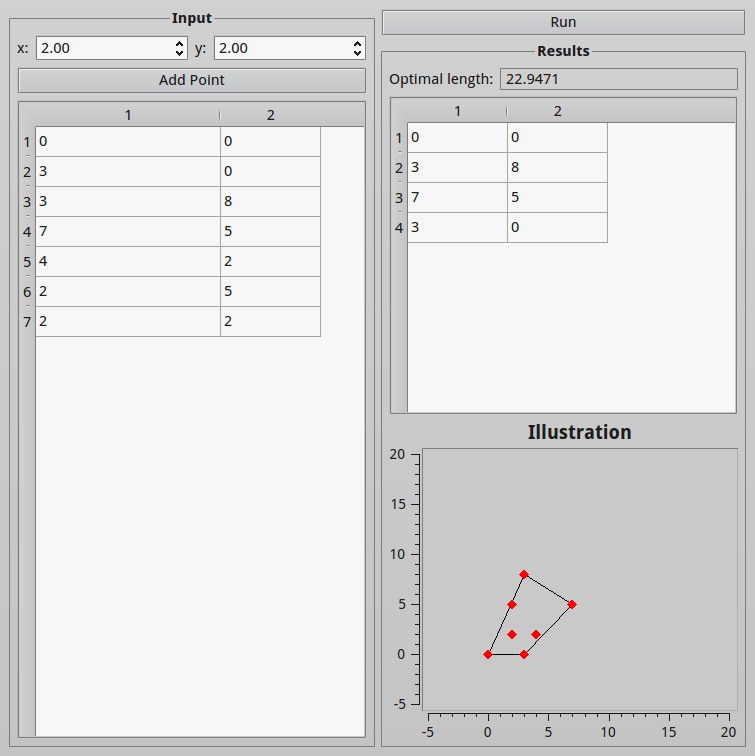
\includegraphics[width=\textwidth]{scr1.png}
  \caption{Розв’язок тестових даних №1}
  \label{fig:f1}
\end{figure}
\paragraph{Тестові дані №2}
\begin{equation}
  A = \left\{ \left( 0; 0 \right), \left( 0; 2 \right), \left( 2; 2
  \right), \left( 2; 0 \right) \right\}
  \label{eq:t2}
\end{equation}
\begin{figure}[h!]
  \centering
  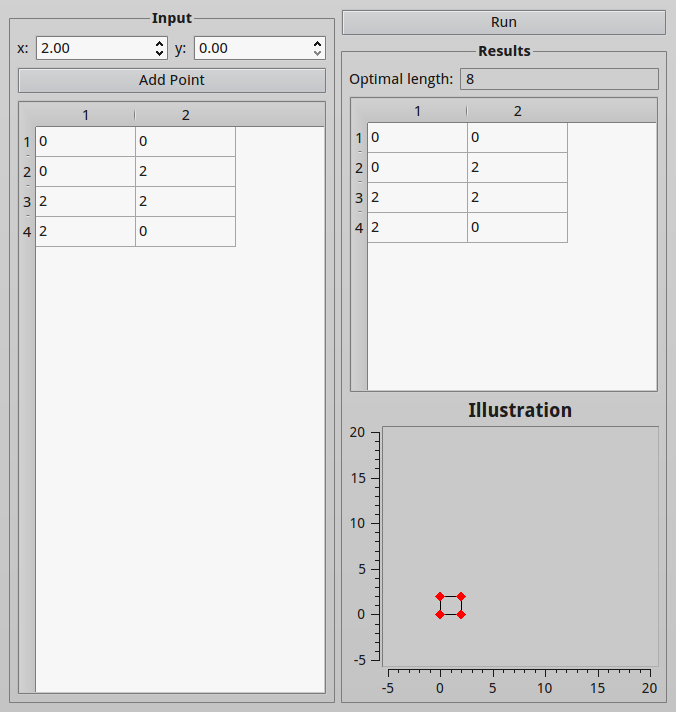
\includegraphics[width=\textwidth]{scr2.png}
  \caption{Розв’язок тестових даних №2}
  \label{fig:f2}
\end{figure}
\paragraph{Тестові дані №3}
\begin{equation}
  A = \left\{ \left( 0; 0 \right), \left( 0; 10 \right), \left( 5; 5
  \right), \left( 10; 10 \right), \left( 10; 0 \right), \left( 5; 15
\right), \left( 5; 10 \right) \right\}
  \label{eq:t3}
\end{equation}
\begin{figure}[h!]
  \centering
  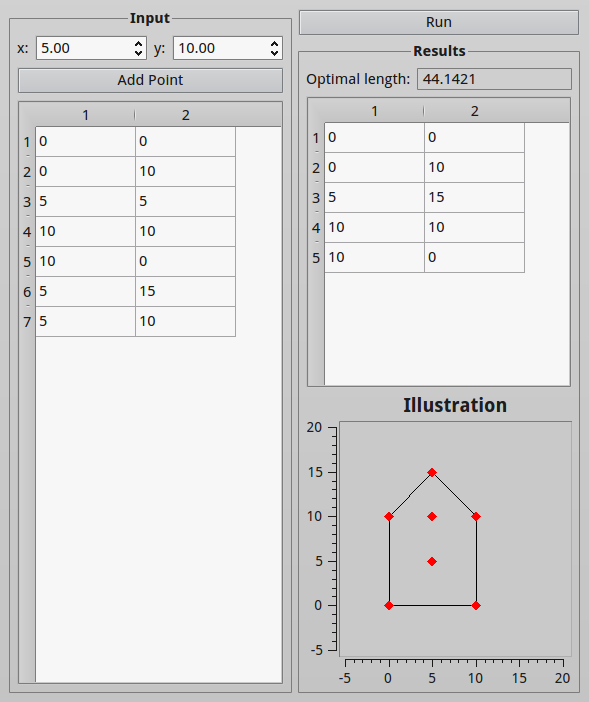
\includegraphics[scale=0.65]{scr3.png}
  \caption{Розв’язок тестових даних №3}
  \label{fig:f3}
\end{figure}

\end{document}
